\subsubsection[Partial Differential Equations, Numerical Analysis]{Partial Differential Equations, \\ Numerical Analysis}
\index{Oliver, Marcel}

\paragraph{Research Team}
Marcel Oliver (Professor), Vladimir Molchanov (PhD Student)

\medskip

% 150 words about research in general

As available computing power continues to increase at a dramatic
pace---approximately following ``Moore's law''---an ever broader range
of systems and natural phenomena is successfully studied by numerical
simulation.  At the same time, it is increasingly apparent that at the
boundaries of different modeling regimes, computations based on the
fundamental laws of physics are, more often than not, under-resolved
in the textbook sense of numerical methods.  Because of the vast range
of scales involved in modeling even seemingly simple systems, this
limitation will not be outgrown by Moore's law within any realistic
time frame.  One therefore has to develop numerical methods and/or
model reductions which capture crucial structures even if the method
is far from ``converging'' in the strong mathematical sense.

My own contributions relate to the preservation of Hamiltonian
structure and, consequently, the retention of relevant conservation
laws under model reduction or numerical discretization.  In fluid
flow, energy cascades to small scales, so that the Hamiltonian picture
must be supplemented by a parametrization of subscale energy
dissipation.  I am working on development and study of rational
subscale closures.


\paragraph{Highlights}

In joint work with Oliver B\"uhler (Courant Institute) I have studied
the closure problem of fluid dynamics in terms of dispersive waves in
Fourier space.  We have demonstrated that this point of view is
fruitful in an idealized model setting: passive advection with smooth
velocity fields.  The closure conditions can then be formulated in
terms of \emph{transparent boundary conditions for lattice waves}.  A
detailed study in the context of simple shear flows has been completed
\cite{OliverBuehler}.  Figure~\ref{fig:OliverBuehler} compares a naive
Galerkin closure, which is conservative and, consequently, contains
artifacts due to ``reflections'' at the truncation boundary in Fourier
space, with the new nonreflecting closure at the same resolution which
approximates the correct behavior very well.  Of course, the Galerkin
closure represents in some sense a worst-case behavior---the point is
that its deficiencies can be understood and eliminated in a rational
and systematic way.  Generalizations of these results to more
realistic modeling scenarios are currently under way.

\begin{figure}[ht]
  \begin{center}
    \fbox{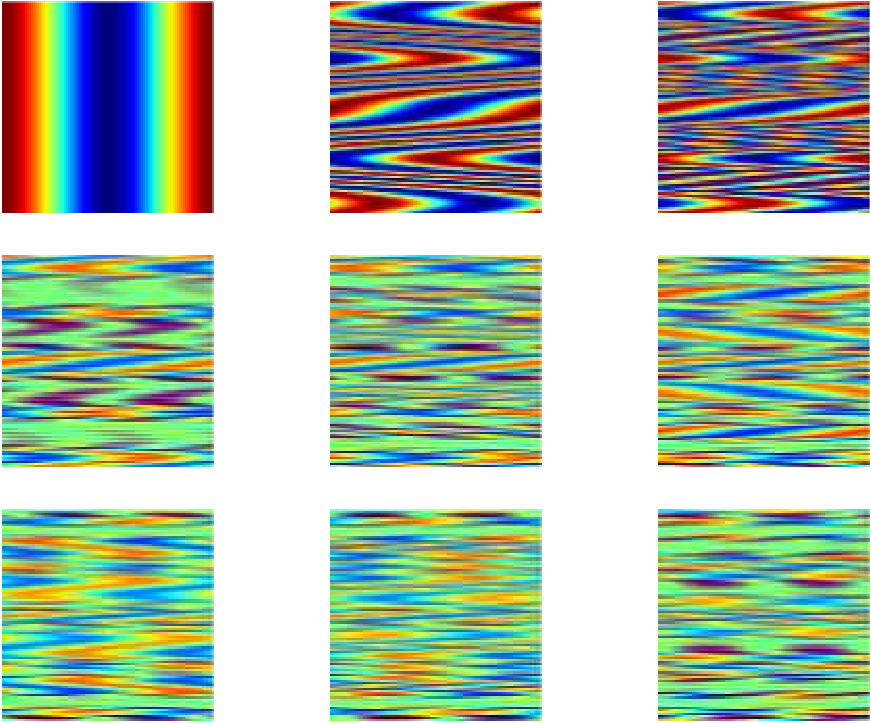
\includegraphics[width=0.45\textwidth]{Oliver/Oliver-Figure1.pdf}} \hfill
    \fbox{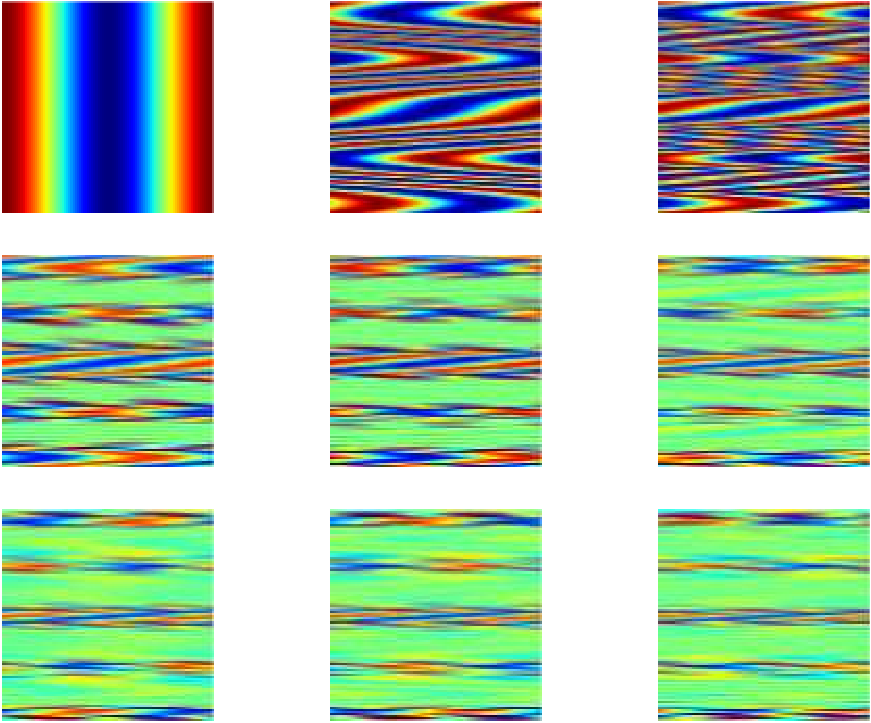
\includegraphics[width=0.45\textwidth]{Oliver/Oliver-Figure2.pdf}} 
    \caption{Evolution of a tracer field in a shear flow.  Shown are
    snapshots at nine different times, with the Galerkin closure top
    and the new transparent closure bottom.}\label{fig:OliverBuehler}
   \end{center}
\end{figure}

So-called symplectic integrators are well known to preserve energy and
other invariants of finite dimensional Hamiltonian systems over very
long times.  This is advantageous in situations where the preservation
of the invariants matters more than strong trajectory accuracy of the
solution.  The approximate preservation of invariants can be
understood in terms of a \emph{backward error analysis} using results
from Hamiltonian normal form theory.  In the context of ordinary
differential equations, this has been known for about 15 years.  But
even for simple partial differential equations, the semilinear wave
equation being a simple relevant model problem in this context, these
classical proofs appear to break down.  In recent work with Claudia
Wulff (Surrey), we have shown that, under somewhat strong assumptions
on the smoothness of the solutions to the semilinear wave equation,
the main features of the finite dimensional theory survive
\cite{OliverWulff}.  We believe that these smoothness assumptions can
still be relaxed by using Lagrangian normal form transformations as we
have successfully applied to model reduction for geophysical fluid flow
in earlier work \cite{Oliver}.  This is current work in progress.

\emph{Particle methods for fluid flow} are a different kind of
structure preserving discretization.  They are especially successful
when flows have huge variations in density, free boundaries, and
changes in domain topology.  There is renewed interest in particle
methods in the context of geophysical fluid flow, primarily because of
the ease with which advected tracer concentrations and
parametrizations of essentially Lagrangian subscale physics can be
built into the model.  While conservation of the various masses is
trivially satisfied, conservation of energy and angular momentum is
not automatic.  In joint work with Onno Bokhove (Twente) we have shown
how rather general fluid models can be reduced to a ``parcel
Hamiltonian formulation'' which provides a reduced Hamilton structure
that, while still in the continuum, survives under a natural
restriction to a finite number of parcels
\cite{BokhoveOliver,BokhoveOliver2}.  My PhD student Vladimir
Molchanov is working on a particular particle method, the Hamiltonian
Particle-Mesh Method of Frank, Gottwald, and Reich.  He has recently
proved that this method converges.  Current work relates to the
question whether his result is sharp, and whether modifications of the
method can yield a better rate of convergence.


\paragraph{Collaborations}
\begin{enumerate}
\item {\sl Twente University, The Netherlands} \\
Dr.\ O. Bokhove \\
Hamiltonian parcel formalism in fluid dynamics.
\item {\sl Courant Institute of Mathematical Sciences, USA} \\
Prof.\ O. B\"uhler \\
Model reductions and model closures in geophysical fluid
dynamics.
\item {\sl University of Michigan, USA} \\
Prof.\ C. Doering \\
Energy growth rates in polymeric channel flows.
\item {\sl Sydney University, Australia} \\
Dr.\ G. Gottwald \\
Multiscale analysis of finite dimensional models of balance.
\item {\sl Heriot--Watt University, UK}
\\ Dr. S. Malham \\
Magnus integrators for eigenvalue problems; Transverse instabilities
in autocatalytic reaction-diffusion systems.
\item {\sl Universit\"at Potsdam, Germany} \\
Prof.\ S. Reich \\
Particle Methods
\item {\sl Surrey University, UK} \\
Dr. C. Wulff \\
Backward error analysis for variational integrators.

\end{enumerate}

\paragraph{Grants}
% list the grants you have received in 2005, if none have been
% received, please delete this 
% subsection. 
\begin{enumerate}
\item {\sl Max--Kade Research Fellowship} to visit the Courant Institute of
Mathematical Sciences, New York, in Spring/Summer 2006
\end{enumerate}

\nocite{GottwaldOliverTecu,GottwaldOliver}
